\documentclass{article}
\usepackage[utf8]{inputenc}
\usepackage{geometry}
\geometry{margin=1in}

\usepackage{graphicx}
\graphicspath{{./images/}}

\usepackage{enumerate}
\usepackage{amssymb}
\usepackage{amsmath}
\usepackage{amsthm}

\begin{document}
\newcommand{\R}{\mathbb{R}}
\newcommand{\claim}{\par\noindent\textit{Claim:}\space}

\setcounter{section}{3}
\section{Continuity}

\begin{enumerate}
\setcounter{enumi}{5}
\item If $f$ is defined on $E$, the \textit{graph} of $f$ is the set of points
      $(x, f(x))$ for $x \in E$ or $E \times f(E)$. In particular, if
      $E \subset \R$ and $f: E \to \R$, then the graph of $f$ is a subset of
      the plane ($\R^2$)

Suppose $E$ is compact. Prove that $f$ is continuous on $E$ if and only if its
graph is compact.

\begin{proof}
Let's first suppose that $f$ is not continuous so there's some $p \in E$ where
$\lim_{x\to p} f(x) \neq f(p)$.

Let $\{p_n\} \to p$ be some sequence of $E$ so that
$\{ f(p_n) \} \to y \in \overline{f(E)}$ where $y \neq f(p)$. Then
$\{ (p_n, f(p_n)) \}$ is an infinite subset of the graph of $f$ which has no
limit point in the graph. This must mean the graph is not compact.

Now suppose that $f$ is continuous. Since $E$ is compact then $f(E)$ is
also compact, and it's trivial to show the cartesian product of two compact sets
is also compact.

\end{proof}

\item If $E \subset X$ and if $f$ is a function defined on $X$, the
      \textit{restriction} of $f$ to $E$ is the function $g$ whose domain of
      definition is $E$, such that $g(p) = f(p)$ for $p \in E$.

Define $f,g : \R^2 \to \R$ as

\[
f(x) =
\begin{cases}
                   0 & (x, y) = (0, 0) \\
\frac{xy^2}{x^2+y^4} & (x, y) \neq (0, 0)
\end{cases},\quad
g(x) =
\begin{cases}
                   0 & (x, y) = (0, 0) \\
\frac{xy^2}{x^2+y^6} & (x, y) \neq (0, 0)
\end{cases}
\]

and prove the following:
\begin{enumerate}[a.]
\item $f$ is bounded on $\R^2$
\item $g$ is unbounded in every neighborhood of $(0, 0)$
\item $f$ is not continuous at $(0, 0)$
\item The restriction of both $f$ and $g$ to any line in $\R^2$ is continuous
\end{enumerate}

\qquad

\begin{enumerate}[a.]
\newcommand{\Boundary}{\frac{1}{2}}

\item \claim $f(x, y) \in [-\Boundary, \Boundary]$ for $(x, y) \in \R^2$.
\begin{proof}
We can equivalently say that $f(x,y) \leq \Boundary$ if $x^2 + y^4 \geq 2xy^2$.
If we plot the functions on either side of the inequality, we can visualize
that the inequality is true ($x^2 + y^4$ is pictured here in orange).

\begin{figure}[h]
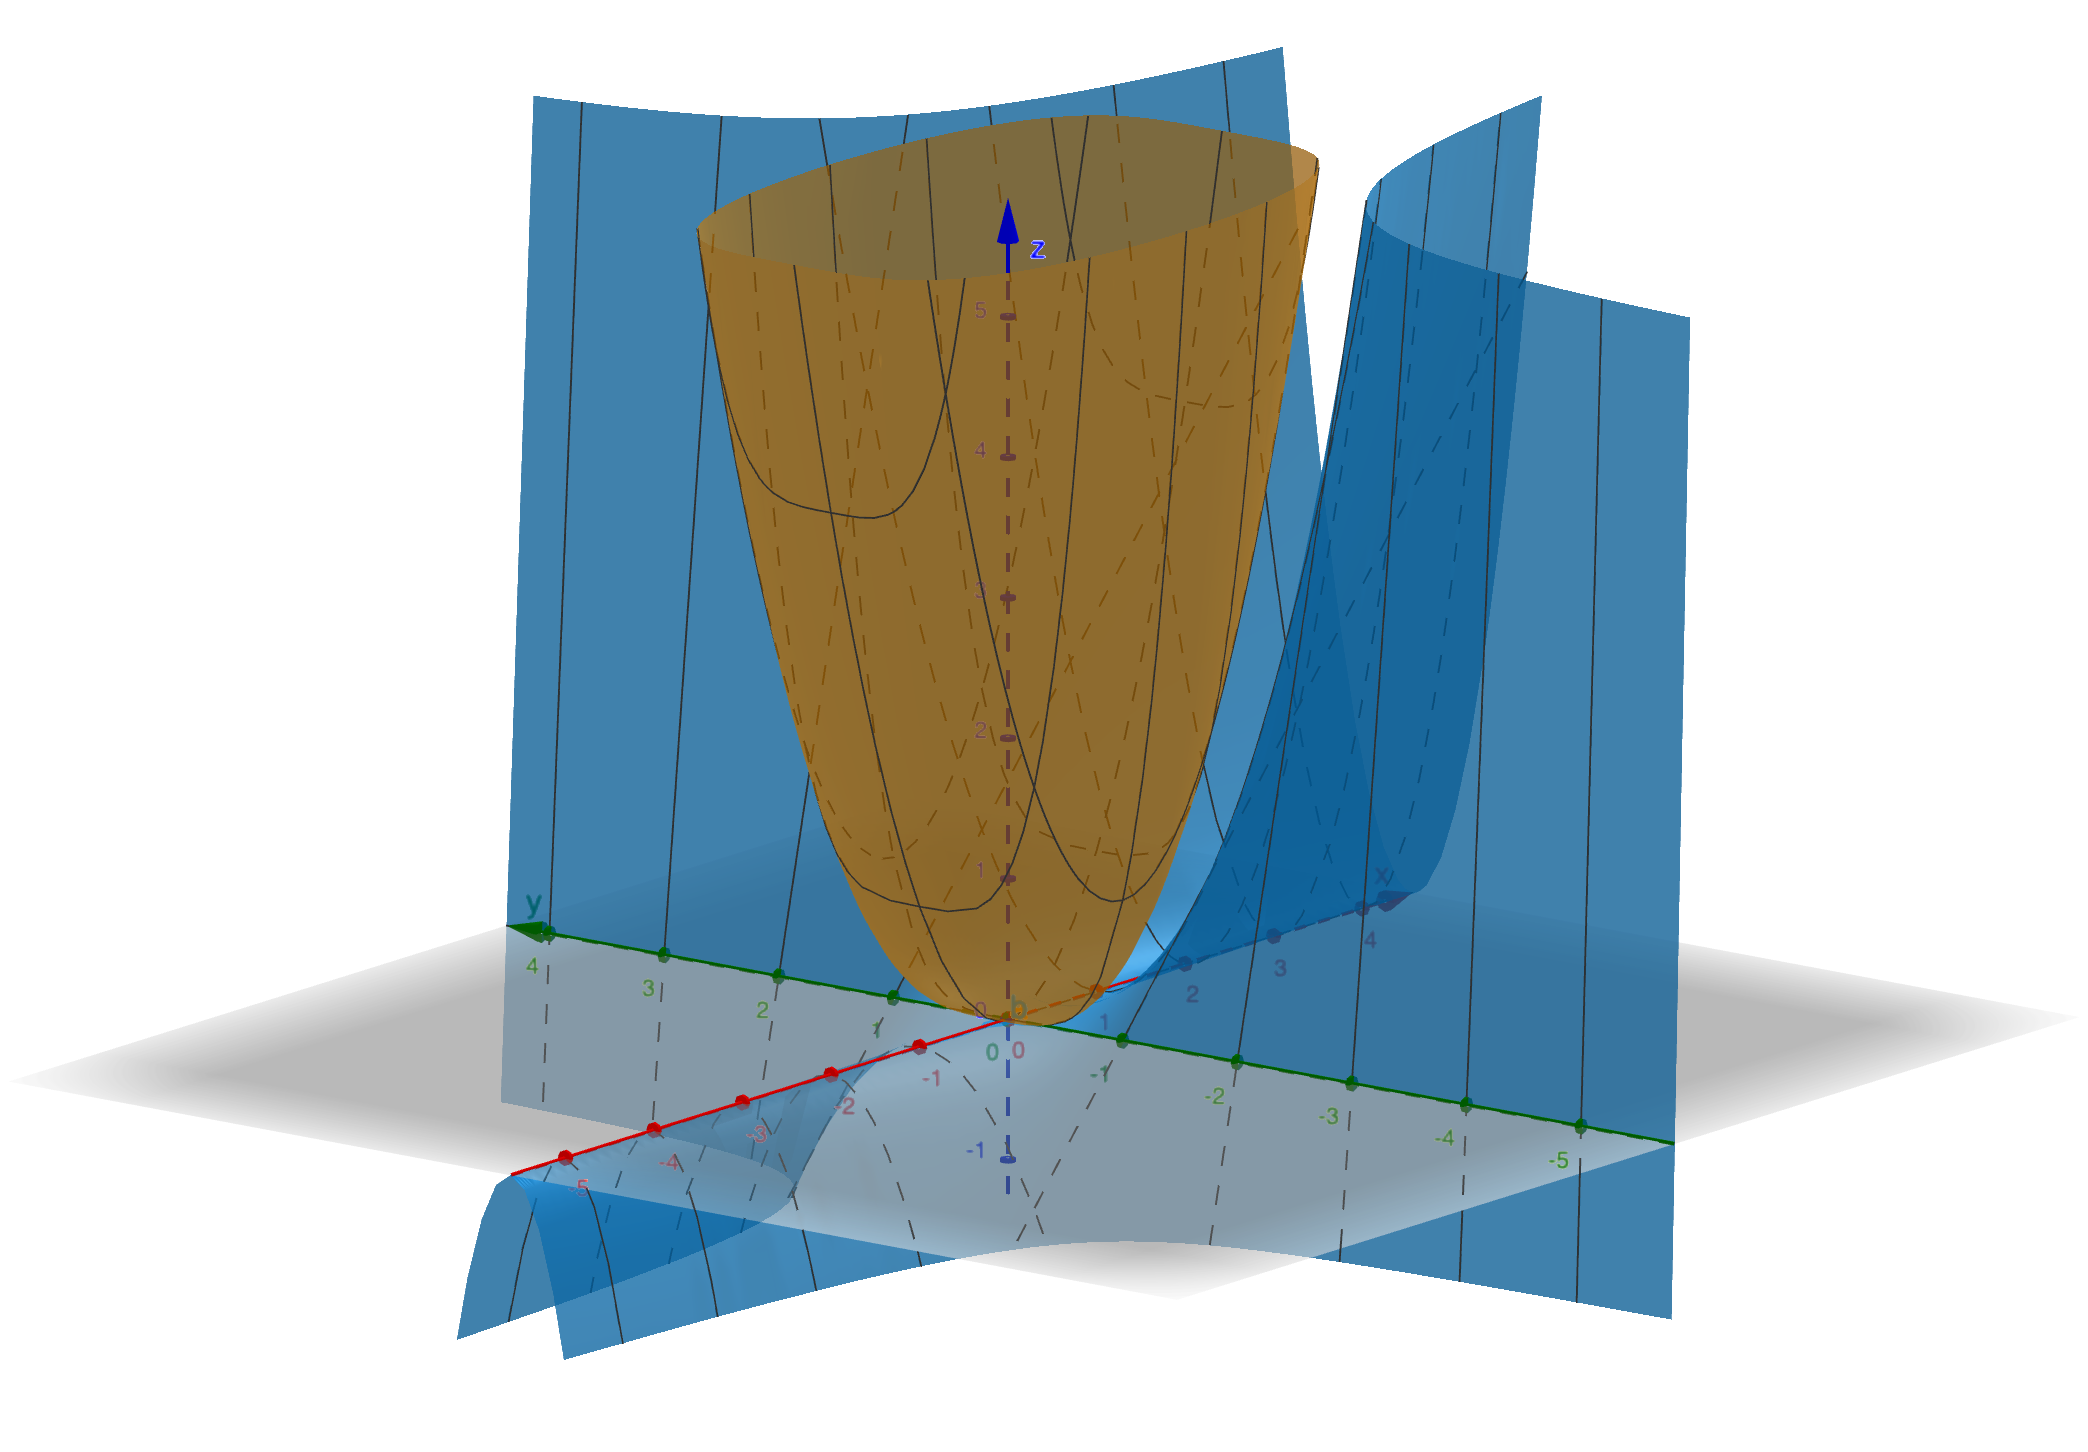
\includegraphics[scale=0.1]{figure-04-07-a}
\centering
\end{figure}

To show this rigorously, let's rearrange the inequality as a quadratic equation
of $y^2$:
\begin{equation*}
\begin{split}
y^4 - 2xy^2 + x^2 &\geq 0 \\
      (y^2 - x)^2 &\geq 0
\end{split}
\end{equation*}
This is clearly true for all $(x, y) \in \R^2$. We can similarly show that
$f(x, y) \geq -\Boundary$ with the statement $(y^2 + x)^2 \geq 0$. This tells
us that $f$ is bounded.
\end{proof}

\item \claim $g$ is unbounded on every neighborhood of $(0, 0)$
\begin{proof}
Once again, visualization can help us construct our proof. If we graph $g$
we can see that a ridge folowing the curve $x^2 = y^6$ grows unbounded as $y$
approaches 0.

\begin{figure}[h]
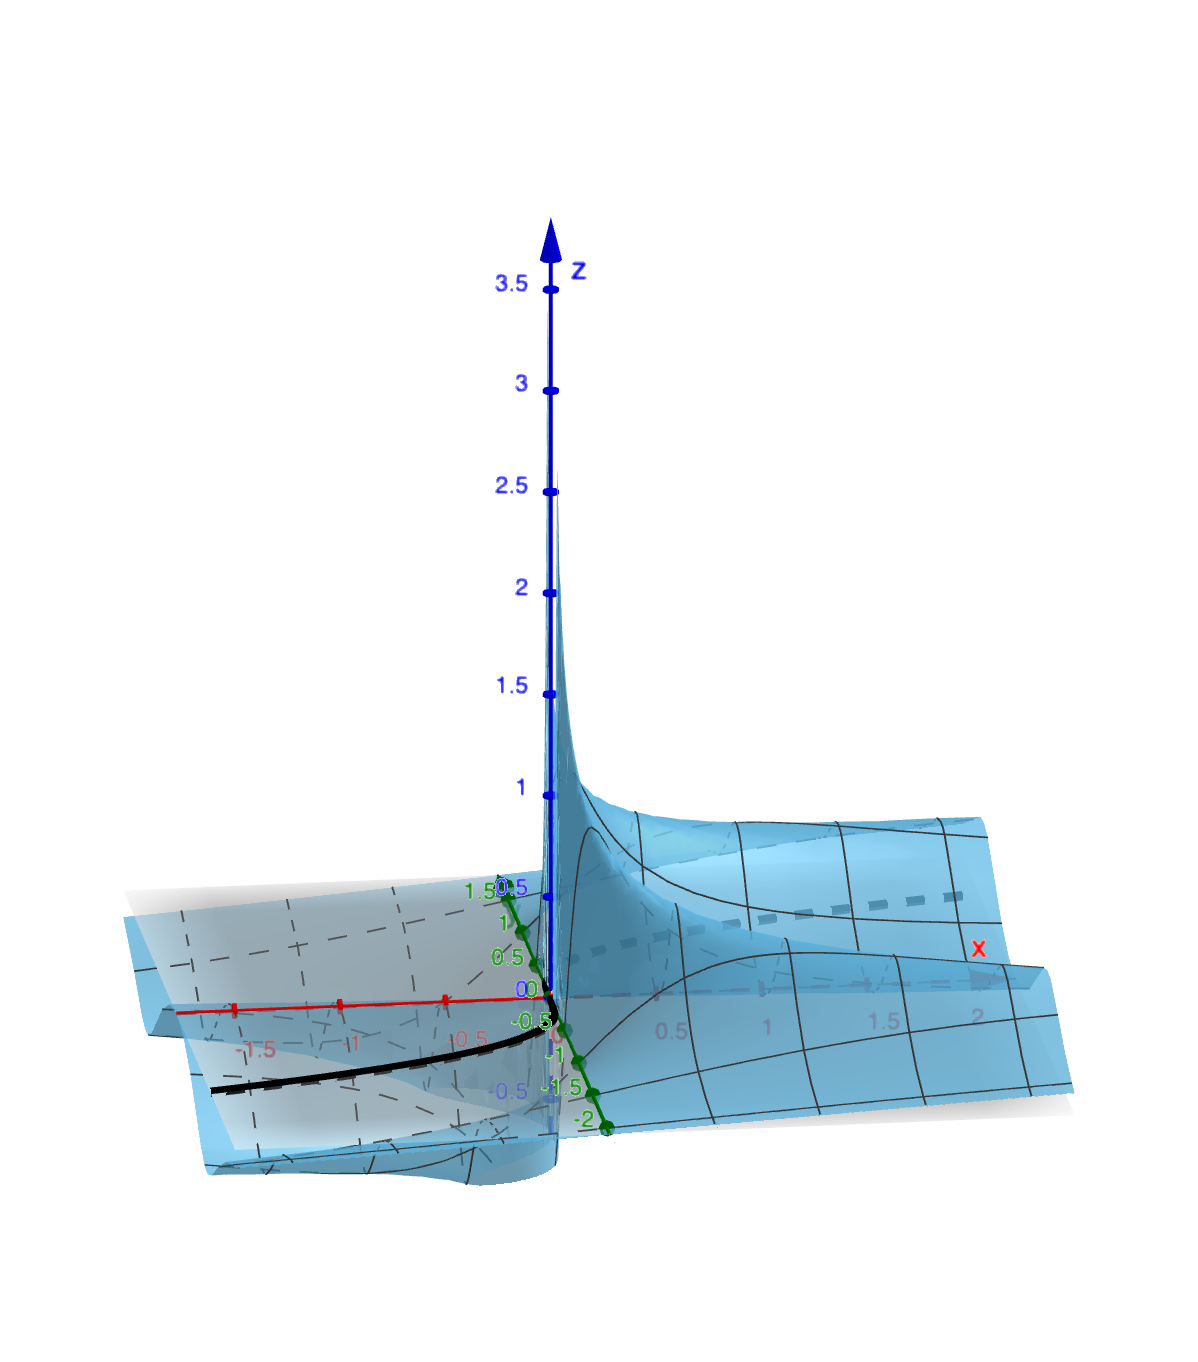
\includegraphics[scale=0.1]{figure-04-07-b1}
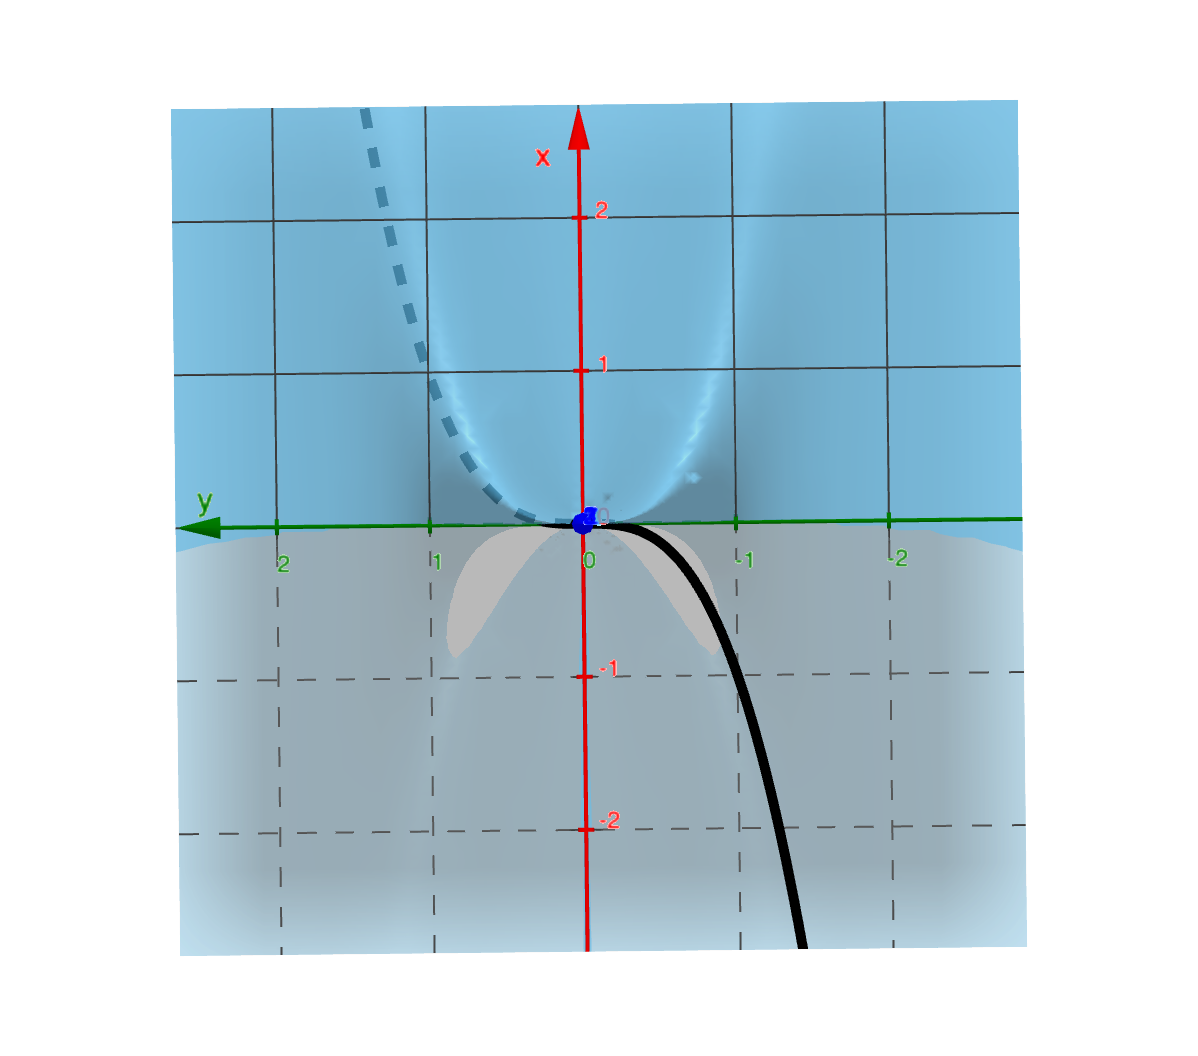
\includegraphics[scale=0.1]{figure-04-07-b2}
\centering
\end{figure}

To show this rigorously, let's construct an unbounded sequence on the graph of
$f$ that follows this unbounded ridge.

Define $p_n = (\frac{1}{n^3}, \frac{1}{n})$ so that $f(p_n) = \frac{n}{2}$.
Let $\epsilon > 0$ be arbitrarily small and let $M > 0$ be arbitrarily large.
If $n \geq 2M$ then $f(p_n) \geq M$. And by the algebraic limit theorem, there's
some $N$ where if $n \geq N$ then $\frac{1}{n^6} + \frac{1}{n^2} < \epsilon^2$.
This shows that $\lvert (\frac{1}{n^3}, \frac{1}{n}) \rvert < \epsilon$. Taking
$n \geq \max \{ 2M, N \}$ shows that $g$ is unbounded on every neighborhood of
$(0, 0)$.
\end{proof}

\item \claim $f$ is not continuous at $(0, 0)$.
\begin{proof}
Similar to our previous problem, let's construct two sequences with the same
limit that follow the curve $x^2 = y^4$, but whose images under $f$ have have
different limits.

Define $p_n = (\frac{1}{n^2}, \frac{1}{n})$ and
$q_n = (-\frac{1}{n^2}, \frac{1}{n})$. Clearly both $p_n \to (0, 0)$ and
$q_n \to (0, 0)$, but $f(p_n) = 1/2$ and $f(q_n) = -1/2$ for all $n$. So clearly
$f$ is not continuous at $(0, 0)$.
\end{proof}

\item \claim The restriction of both $f$ and $g$ to any line in $\R^2$ is
      continuous.

\begin{proof}
Let $c, m \in \R$ so that $y = mx + b$ defines an arbitrary line in $\R^2$.
By the algebraic limit theorem, $f(x, mx + b)$ and $g(x, mx+b)$ are both
continuous if their denominators are nonzero. So then let's show the
denominators are always nonzero.

If $b = 0$ then $x^2$ can be factored out of both fractions to get
\begin{equation*}
f(x, mx) = \frac{m^2x}{1+m^4x^2}, \qquad g(x, mx) = \frac{m^2x}{1+m^6x^4}
\end{equation*}
The even powers in the denominator mean variable term in the denominator must be
non-negative, and the constant 1 ensures the denominator is nonzero.

A similar argument shows that holding $y$ or $x$ constant gives a nonzero
denominator:

\begin{equation*}
\begin{split}
f(x, b) = \frac{b^2x}{x^2 + b^4}, &\qquad f(b, y) = \frac{by^2}{y^4 + b^2} \\
g(x, b) = \frac{b^2x}{x^2 + b^6}, &\qquad g(b, y) = \frac{by^2}{y^6 + b^2}
\end{split}
\end{equation*}

If $b,m$ are nonzero then consider $h(x) = x^2 + (mx + b)^{2k}$. If $x = -m/b$
then $h(x) = m^2/b^2$. If $x \neq -m/b$ then $(mx +b)^{2k} > 0$ and so $h(x)$
is always nonzero.
\end{proof}
\end{enumerate}

\item Let $E \subset \R$ be bounded, and let $f: E \to \R$ be uniformly
      continuous.

\claim $f(E)$ is also bounded.
\begin{proof}
If $E$ has no limit points then $E$ must be finite since it's bounded. This must
also mean $f(E)$ is bounded. Now suppose $E$ at least one limit point.

Let $p$ be any limit point of $E$ and suppose for contradiction that $f(x)$
grows unbounded as $x \to p$. Let $\delta > 0$ and choose some $q \in E$ where
$| p - q | < \delta$. Put $M = |f(q)|$.

Since $f(x)$ is unbounded as $x \to P$, there must be some $s \in E$ where
$| p - s | < \delta$ and $|f(s)| \geq M + 1$. Then $| p - q | < \delta$, but
$| f(p) - f(q) | \geq 1/2$, which contradicts that $f$ is uniformly continuous.
\end{proof}

Taking $f(x) = x$ shows that $f$ need not be bounded if $E$ is unbounded.
\end{enumerate}

\end{document}
